%% ------------------------------------------------------------------------- %%
\chapter{Experimentos}
\label{cap:experimentos}
Este capítulo é dividido em quatro momentos distintos dos experimentos realizados
para esta monografia. Primeiro, na Seção \ref{sec:powerworkflowsim} é
apresentado o simulador desenvolvido para esta monografia, o PowerWorkflowSim;
Depois, na Seção \ref{sec:ambiente_simulado} são
apresentadas as configurações do ambiente experimental; Resultados dos 
experimentos de controle são exibidos na Seção \ref{sec:experimentos-controle}.
Em seguida, na Seção
\ref{sec:algoritmo_proposto} é feito um estudo detalhado sobre a heurística
proposta para minimizar o consumo energético e o algoritmo correspondente
implementado; Por fim na Seção \ref{sec:resultados_experimentais} são
apresentados os resultados experimentais que mostram o ganho energético com
o uso do algoritmo proposto.

\section{PowerWorkflowSim}
\label{sec:powerworkflowsim}
Durante a implementação do WorkflowSim os desenvolvedores não tomaram o cuidado
de manter a API de simulação energética do CloudSim acessível ao usuário final.
De maneira a resolver esse problema, o autor da monografia desenvolveu uma versão
alternativa do WorkflowSim, o PowerWorkflowSim.

Como tanto a API energética do CloudSim quanto o WorkflowSim são basicamente 
\emph{wrappers} do CloudSim, o trabalho necessário foi o de garantir que 
a funcionalidade de um não conflitasse com a do outro. O diagrama de classes
resultante do PowerWorkflowSim está representado abaixo.

\begin{figure}[ht]
\centering
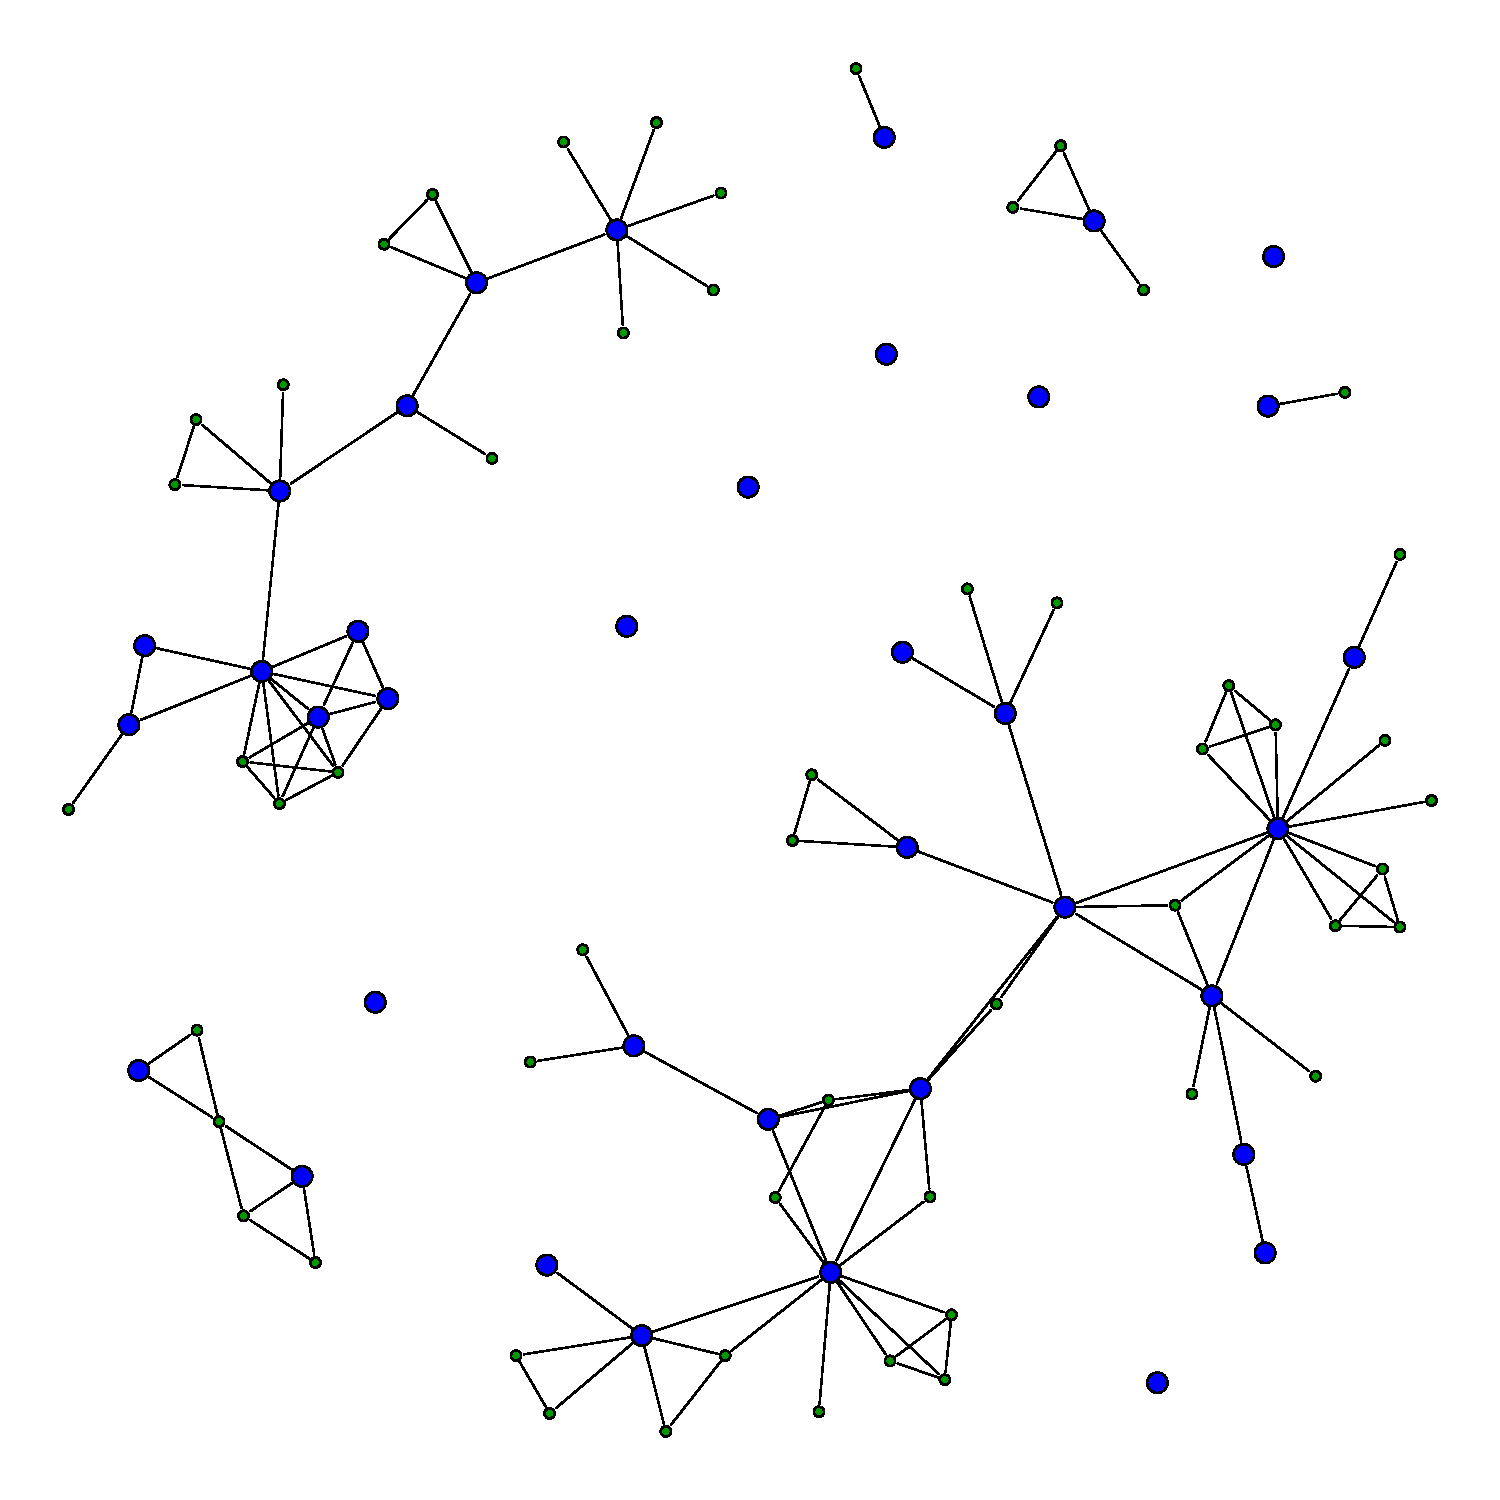
\includegraphics[draft,width=8cm,height=5cm]{graph.pdf}
\caption{Diagrama de Classes do PowerWorkflowSim}
\label{fig:classes_powerworkflowsim}
\end{figure}


\section{Ambiente Simulado}
\label{sec:ambiente_simulado}
%\subsection{Máquina Virtual}
Esta seção apresenta os valores adotados para os diversos parâmetros disponíveis
a uma simulação do PowerWorkflowSim. As configurações estão divididas
por entidades: Na Tabela \ref{tab:configuracao_vm} são apresentadas as
configurações de uma máquina virtual. Já nas Tabelas \ref{tab:configuracao_hp_g3}
e \ref{tab:configuracao_hp_g5} estão presentes as configurações das máquinas
físicas simuladas, duas versões de servidores HP ProLiant ML110, um da geração 3
e outro da geração 5. Ainda, na Tabela \ref{tab:configuracao_datacenter} são
apresentadas as configurações que abrangem o Datacenter simulado. Por fim,
na Tabela \ref{tab:configuracao_powerworkflowsim} são vistas as configurações
do simulador como um todo.

\begin{savenotes}
\begin{table}
	\centering
    \begin{tabular}{|c|c|}
    \hline
    \textbf{Parâmetro}     & \textbf{Valor}     \\ \hline
    Número de máquinas     & 20        \\
    Número de \emph{Cores} & 1         \\
    Velocidade de um Core  & 1000 MIPS \\
    Tamanho da Imagem      & 10 GB  \\
    RAM                    & 512 MB    \\
    Largura de Banda       & 1 Gbps \\
    Gerenciamento de tarefas & Compartilhadas no espaço\footnote{Tarefas
    compartilhadas no espaço possuem fatias do recurso desejado
    reservadas a cada uma delas. Outra alternativa é o compartilhamento no tempo
    no qual cada tarefa faz uso de dos recursos por uma fatia de tempo
    determinada em esquema \emph{round-robin}, por exemplo.} \\
    Gerenciador de VMs     & Xen       \\     \hline
    \end{tabular}
    \caption {Configurações das máquinas virtuais}
    \label{tab:configuracao_vm}
\end{table}
\end{savenotes}

%\subsection{\emph{Host}}
\begin{table}
	\centering
    \begin{tabular}{|c|c|}
    \hline
    \textbf{Parâmetro}            & \textbf{Valor}     \\ \hline
    Número de máquinas            & 10                            \\
    Número de \emph{Cores}        & 2                             \\
    Velocidade de um Core         & 1860 MIPS (Xeon 3040)         \\
    RAM                           & 4 GiB                         \\
    Largura de Banda              & 1 Gbps                        \\
    Armazenamento                 & 1 GB                          \\
    Modelo de consumo energético  & \cite{spec:proliant_ml110_g3} \\ \hline
    \end{tabular}
    \caption {Configuração de um host HP ProLiant ML110 G3}
    \label{tab:configuracao_hp_g3}
\end{table}



\begin{table}
	\centering
    \begin{tabular}{|c|c|}
    \hline
    \textbf{Parâmetro}            & \textbf{Valor}     \\ \hline
    Número de máquinas            & 10                            \\
    Número de \emph{Cores}        & 2                             \\
    Velocidade de um Core         & 2660 MIPS (Xeon 3075)         \\
    RAM                           & 4 GiB                         \\
    Largura de Banda              & 1 Gbps                        \\
    Armazenamento                 & 1 GB                          \\
    Modelo de consumo energético  & \cite{spec:proliant_ml110_g5} \\ \hline
    \end{tabular}
    \caption {Configuração de um \emph{host} HP ProLiant ML110 G5}
    \label{tab:configuracao_hp_g5}
\end{table}

%\subsection{\emph{Datacenter}}

\begin{savenotes}
\begin{table}
	\centering
    \begin{tabular}{|c|c|}
    \hline
    \textbf{Parâmetro}     & \textbf{Valor}     \\ \hline
    Arquitetura            & x86          \\
    Sistema Operacional    & Linux        \\
    Gerenciador de VMs     & Xen          \\
    Fuso Horário           & -3           \\
    Custo de Processamento & 3 unidades\footnotemark[2]   \\
    Custo da RAM           & 0.05 unidade\footnotemark[2]  \\
    Custo do Armazenamento & 0.1 unidade\footnotemark[2]  \\
    Custo da Banda         & 0.1 unidade\footnotemark[2]  \\ \hline
    \end{tabular}
    \caption {Configurações do \emph{datacenter}}
    \label{tab:configuracao_datacenter}
\end{table}
\end{savenotes}
\footnotetext[2]{Custo medido em unidades monetárias, reais por exemplo, para
alocar uma máquina com esta configuração. Com este valor é possível
implementar políticas de alocação de máquinas virtuais mais ou menos baratas
para executar uma determinada tarefa.}


%\subsection{Parâmetros do WorkflowSim}
\begin{table}
	\centering
    \begin{tabular}{|c|c|}
    \hline
    \textbf{Parâmetro}                & \textbf{Valor}     \\ \hline
    Escalonador                       & \emph{First Come First Served}    \\
    Estratégia de Economia de Energia & DVFS (Vide Seção \ref{subsec:dvfs}) \\ \hline
    \end{tabular}
    \caption {Configurações do PowerWorkflowSim}
    \label{tab:configuracao_powerworkflowsim}
\end{table}


\section{Experimentos de controle}
\label{sec:experimentos-controle}
Para facilitar a análise de algoritmos que operam sobre fluxos de trabalho,
tais como os algoritmos descritos nesta monografia, o projeto Pegasus Workflow
Management System desenvolveu uma ferramenta geradora de \emph{workflows}
científicos. Estes \emph{workflows} artificiais são gerados a partir de
informações extraídas de instâncias reais das aplicações juntamente com
conhecimentos prévios sobre seu funcionamento interno
\cite{pegasus:workflowgenerator}.

Os fluxos gerados pelo projeto Pegasus foram então executados no
PowerWorkflowSim com as configurações apresentadas na Seção 
\ref{sec:ambiente_simulado}. Os resultados são apresentados na Tabela 
\ref{tab:resultados_dvfs}.

\begin{table}
	\centering
    \begin{tabular}{|c|c|c|c|}
    \hline
    \textbf{Experimento}           & \textbf{Número de tarefas} & \textbf{Tempo simulado (s)} & \textbf{Consumo energético (kWh)} \\ \hline
    CyberShake                     & 30                & 246.65             & 0.13                     \\
    CyberShake                     & 50                & 267.20             & 0.15                     \\
    CyberShake                     & 100               & 306.94             & 0.17                     \\
    CyberShake                     & 1000              & 1265.71            & 0.69                     \\ \hline
    Epigenomics                    & 24                & 5596.59            & 3.04                     \\
    Epigenomics                    & 46                & 7743.25            & 4.20                     \\
    Epigenomics                    & 100               & 34975.01           & 18.99                    \\
    Epigenomics                    & 997               & 207426.20          & 112.62                   \\ \hline
    Inspiral                       & 30                & 1335.62            & 0.73                     \\
    Inspiral                       & 50                & 1411.25            & 0.77                     \\
    Inspiral                       & 100               & 1519.47            & 0.82                     \\
    Inspiral                       & 1000              & 11712.90           & 6.36                     \\ \hline
    Montage                        & 25                & 46.99              & 0.03                     \\
    Montage                        & 50                & 66.76              & 0.04                     \\
    Montage                        & 100               & 102.91             & 0.06                     \\
    Montage                        & 1000              & 907.13             & 0.49                     \\ \hline
    Sipht                          & 30                & 4412.76            & 2.40                     \\
    Sipht                          & 60                & 4642.49            & 2.52                     \\
    Sipht                          & 100               & 4479.34            & 2.43                     \\
    Sipht                          & 1000              & 9646.45            & 5.24                     \\ \hline
    \end{tabular}
    \caption {Resultados dos experimentos de controle}
    \label{tab:resultados_dvfs}
\end{table}



\section{Algoritmo Proposto}
\label{sec:algoritmo_proposto}

\section{Resultados Experimentais}
\label{sec:resultados_experimentais}

